
\section{Introduction}
The prevalence of positioning devices has drastically boosted 
the scale and spectrum of trajectory collection to an unprecedented level. 
Tremendous amounts of trajectories, in the form of sequenced spatial-temporal 
records, are continually generated from animal telemetry chips, 
vehicle GPSs and wearable devices. Data analysis on large-scale 
trajectories benefits a wide range of applications and services, 
including traffic planning~\cite{zheng2011urban}, animal analysis~\cite{li2010miningperiodic}, and social recommendations~\cite{bao2013survey}, to name just a few.


A crucial task of data analysis on top of trajectories is 
to discover co-moving patterns. A \emph{co-movement} pattern~\cite{li2013managing} 
refers to a group of objects traveling together for a certain period of time 
and the group is normally determined by spatial proximity. 
A pattern is prominent if the size of the group exceeds $M$ and the length of the duration exceeds $K$, where $M$ and $K$ are parameters specified by users. Rooted from such basic definition 
and driven by different mining applications, there are a bunch of variants 
of co-movement patterns that have been developed with more advanced constraints.

Table~\ref{tbl:existing_co_patterns} summarizes several popular co-moving pattern s 
with different constraints in the attributes of clustering in spatial proximity,
consecutiveness in temporal duration and computational complexity. 
In particular,  the \emph{flock}~\cite{gudmundsson2006flock} 
and the \emph{group}~\cite{wang2006grouppattern} patterns require 
all the objects in a group to be enclosed by a disk with radius $r$; 
whereas the \emph{convoy}~\cite{jeung2008convoy}, the \emph{swarm}~\cite{li2010swarm} 
and the \emph{platoon}~\cite{li2015platoon} patterns resort to density-based 
spatial clustering. 
In the temporal dimension, the \emph{flock}~\cite{gudmundsson2006flock} 
and the \emph{convoy}~\cite{jeung2008convoy} require all the timestamps 
of each detected spatial group to be consecutive, which is referred to as \emph{global consecutiveness}; 
whereas the \emph{swarm}~\cite{li2010swarm} does not impose any restriction. 
The \emph{group}~\cite{wang2006grouppattern} and the \emph{platoon}~\cite{li2015platoon} adopt a compromised manner by allowing
arbitrary gaps between the consecutive segments, which is called \emph{local consecutiveness}. 
They introduce a parameter $L$ to control the minimum length of each local consecutive segment.


\begin{table} \scriptsize
\centering
\begin{tabular}{|c|c|c|c|}
\hline 
Patterns & {\tiny Proximity} & {\tiny Consecutiveness} & {\tiny Time Complexity}\\ 
\hline 
flock~\cite{gudmundsson2004flock} & disk-based &  global & $O(|\mathbb{O}||\mathbb{T}|(M + log(|\mathbb{O}|))$ \\ 
\hline 
convoy~\cite{jeung2008convoy} & density-based &   global & $O(|\mathbb{O}|^2+|\mathbb{O}||\mathbb{T}|)$\\ 
\hline 
swarm~\cite{li2010swarm} & density-based  & - & $O(2^{|\mathbb{O}|}|\mathbb{O}||\mathbb{T}|)$  \\ 
\hline 
group~\cite{wang2006grouppattern} & disk-based &  local & $O(|\mathbb{O}|^2|\mathbb{T}|)$ \\ 
\hline 
platoon~\cite{li2015platoon} & density-based &  local & $O(2^{|\mathbb{O}|}|\mathbb{O}||\mathbb{T}|)$\\ 
\hline 
\end{tabular} 
\caption{Constraints and complexity of co-movement patterns. The time complexity indicates the performance in the worst case, where $|\mathbb{O}|$ is the total number of objects and $|\mathbb{T}|$ is the number of descritized timestamps.}
\label{tbl:existing_co_patterns}
\end{table}




\begin{figure}[h]
\centering
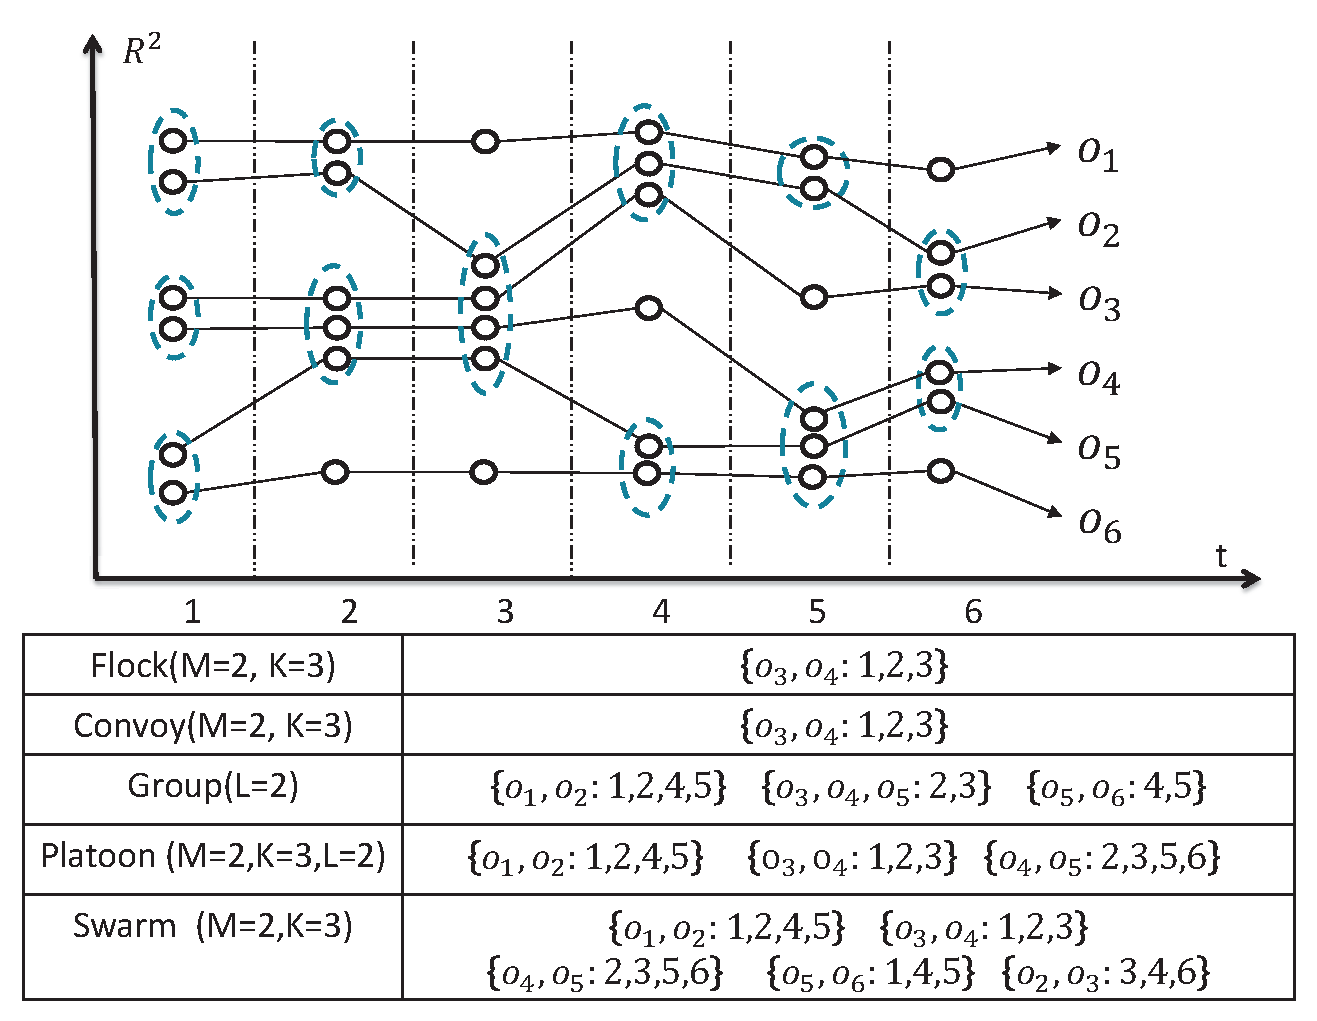
\includegraphics[width=0.45\textwidth]{related_work.eps}
\caption{Trajectories and co-movement patterns; The example consists of six trajectories across six snapshots. Objects in spatial clusters are enclosed by dotted circles. $M$ is the minimum cluster cardinality; $K$ denotes the minimum number of snapshots for the occurrence of a spatial cluster; and $L$ denotes the minimum length for local consecutiveness.}
\label{fig:related_work}
\end{figure}

Figure~\ref{fig:related_work} is an example to demonstrate the concepts of various co-movement patterns. The trajectory database consists of six moving objects and the temporal dimension is discretized into six snapshots. In each snapshot, we treat the clustering methods as a black-box and assume that they generate the same clusters. Objects in proximity are grouped in the dotted circles. As aforementioned, there are three parameters to determine the co-movement patterns and the default settings in this example are $M=2$, $K=3$ and $L=2$. Both the \emph{flock} and the \emph{convoy} require the spatial clusters to last for at least $K$ consecutive  timestamps. Hence,$\{o_3,o_4\}$ and $\{o_5,o_6\}$  remains the only two candidates matching the patterns. The \textit{swarm} relaxes the pattern matching by discarding the temporal consecutiveness constraint. Thus, it generates many more candidates than the \textit{flock} and the \textit{convoy}. The \textit{group} and the \textit{platoon} add another constraint on local consecutiveness to retain meaningful patterns. For instance, $\{o_1,o_2:1,2,4,5\}$ is a pattern matching local consecutiveness because timestamps $\{1,2\}$ and $\{4,5\}$ are two segments with length no smaller than $L=2$. The difference between the \textit{group} and the \textit{platoon} is that the \textit{platoon} has an additional parameter $K$ to specify the minimum number of snapshots for the spatial clusters. This explains why $\{o_3,o_4,o_5:2,3\}$ is a  \textit{group} pattern but not a \textit{platoon} pattern.

As can be seen, there are various co-movement patterns requested by different applications and it is cumbersome to design a tailored solution for each type. In addition, despite the generality of the \emph{platoon} (i.e., it can be reduced to other types of patterns via proper parameter settings), it suffers from the so-called \emph{loose-connection} anomaly. We use two objects $o_1$ and $o_2$ in Figure~\ref{fig:platoon_weakpoint} as an example to illustrate the scenario. These two objects form a \emph{platoon} pattern in timestamps $\{1,2,3,102,103,104\}$. However, the two consecutive segments are $98$ timestamps apart, resulting in a false positive co-movement pattern. In reality, such an anomaly may be caused  by the periodic movements of unrelated objects, such as vehicles stopping at the same petrol station or animals pausing at the same water source. 
Unfortunately, none of the existing patterns have directly addressed this anomaly.


%As can be seen, there are various co-movement patterns requested by different 
%applications and it is cumbersome to design a tailored solution for each type. 
%As pointed in \cite{li2015platoon, li2010swarm}, stringent temporal constraints (e.g., global consecutiveness on \emph{flock} and \emph{convoy}) may miss out many interesting patterns. However, we 
%further observe that pattern definitions with overly-relaxed temporal constraints (e.g., \emph{swarm}, \emph{group} and \emph{platoon}) lose the fine control of a pattern which lead to noisy results and unnecessary computations. We name this scenario as \emph{loose-connection} anomaly. To illustrate, as shown in Figure~\ref{fig:platoon_weakpoint}, the two objects $o_1, o_2$ form a \emph{platoon} pattern 
%$\{o_1,o_2:1,2,3,102,103,104\}$. However, the consecutive segments are $98$ timestamps apart, 
%making the co-moving behavior very loose.
%In reality, such an anomaly is likely induced by the periodic movements of unrelated objects 
%such as, vehicles stopping at the same petrol station, animals pausing at the same water source etc.  Interestingly, none of the temporal-relaxed patterns (e.g., \emph{swarm}, \emph{group} and \emph{platoon}) are able to directly avoid such an anomaly.

%In addition, existing pattern definitions are not expressive enough and may miss 
%interesting patterns or return noisy results. We summarize 
%the two scenarios as \emph{missing-pattern} anomaly
%and \emph{loose-connection} anomaly.
%A \emph{missing-pattern} anomaly arises due to the stringent constraints on the pattern duration.
%As shown in Figure~\ref{fig:platoon_weakpoint} (a), if we set $K=4$, 
%neither \emph{flock}s nor \emph{convoy}s can be discovered. This is because
%$o_1$ is away from $o_2$ at timestamp $4$, which is likely caused by
%the traffic control or the clustering inaccuracy at time $4$. On the other hand,
%the \emph{loose-connection} anomaly occurs due to an over-relaxed constraint on 
%the duration. As shown in Figure~\ref{fig:platoon_weakpoint} (b),
%the two objects $o_1, o_2$ form a \emph{platoon} pattern 
%$\{o_1,o_2:1,2,3,102,103,104\}$. However, the consecutive segments are $98$ timestamps apart, 
%making the co-moving behavior very weak.
%In reality, such an anomaly is likely to be induced by the periodic movements of unrelated objects 
%such as, vehicles stopping at the same petrol station, animals pausing at the same water source etc. 
%It is easy to see that none of the existing co-movement patterns are able to avoid these two anomalies.

\begin{figure}[h]
\center
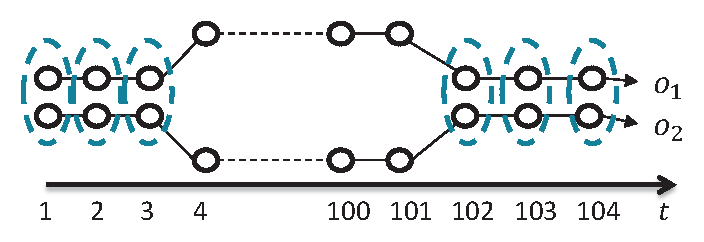
\includegraphics[width=0.35\textwidth]{platoon_weakpoint.eps}
\caption{\emph{Loose-connection} anomaly. Even though $\{o_1, o_2: 1,2,3,102,103,104\}$ is considered as a valid \emph{platoon} pattern, it is highly probable that these two objects are not related as the two consecutive segments  are 98 timestamps apart. 
% in \emph{platoon}, \emph{swarm} and \emph{group} results.
}
\label{fig:platoon_weakpoint}
\end{figure}

%In current literature,
%users are unable to explicitly exclude the loosely-connected patterns even when those patterns are unwanted.
%
%
% we summarize two anomalies 
%The \emph{missing-pattern}~\cite{li2010swarm} anomaly arises due to the stringent constraints on the duration of a pattern. As shown in 
%Figure~\ref{fig:platoon_weakpoint} (a).  As we notice, object $o_1$ is temporally far from $o_2$ at timestamp $4$, which is likely to be
%the result of errors in interpretation of missing points, or $o_1$ faces traffic control at time $4$. Such an anomaly can
%be resolved by \emph{swarm} and \emph{platoon} due to a relaxed constraint on the duration. However, 
%\emph{swarm} and \emph{platoon}'s relaxations encompass a type of non-interesting patterns which is referred
%as \emph{loose-connection}~\cite{li2015platoon} anomaly. 
%
%
%%This is because that \emph{platoon} allows the timestamps in a pattern duration to be in arbitrary distance, making the object group loosely
%connected. For instance, patterns with duration $\{1,2,100,101\}$ could be a valid \emph{platoon}; however, the two timestamps $2,100$ are too far from each other.

%For instance, PUT THE FIGURE AND EXPLANATION HERE.

%\begin{figure}[h]
%\center
%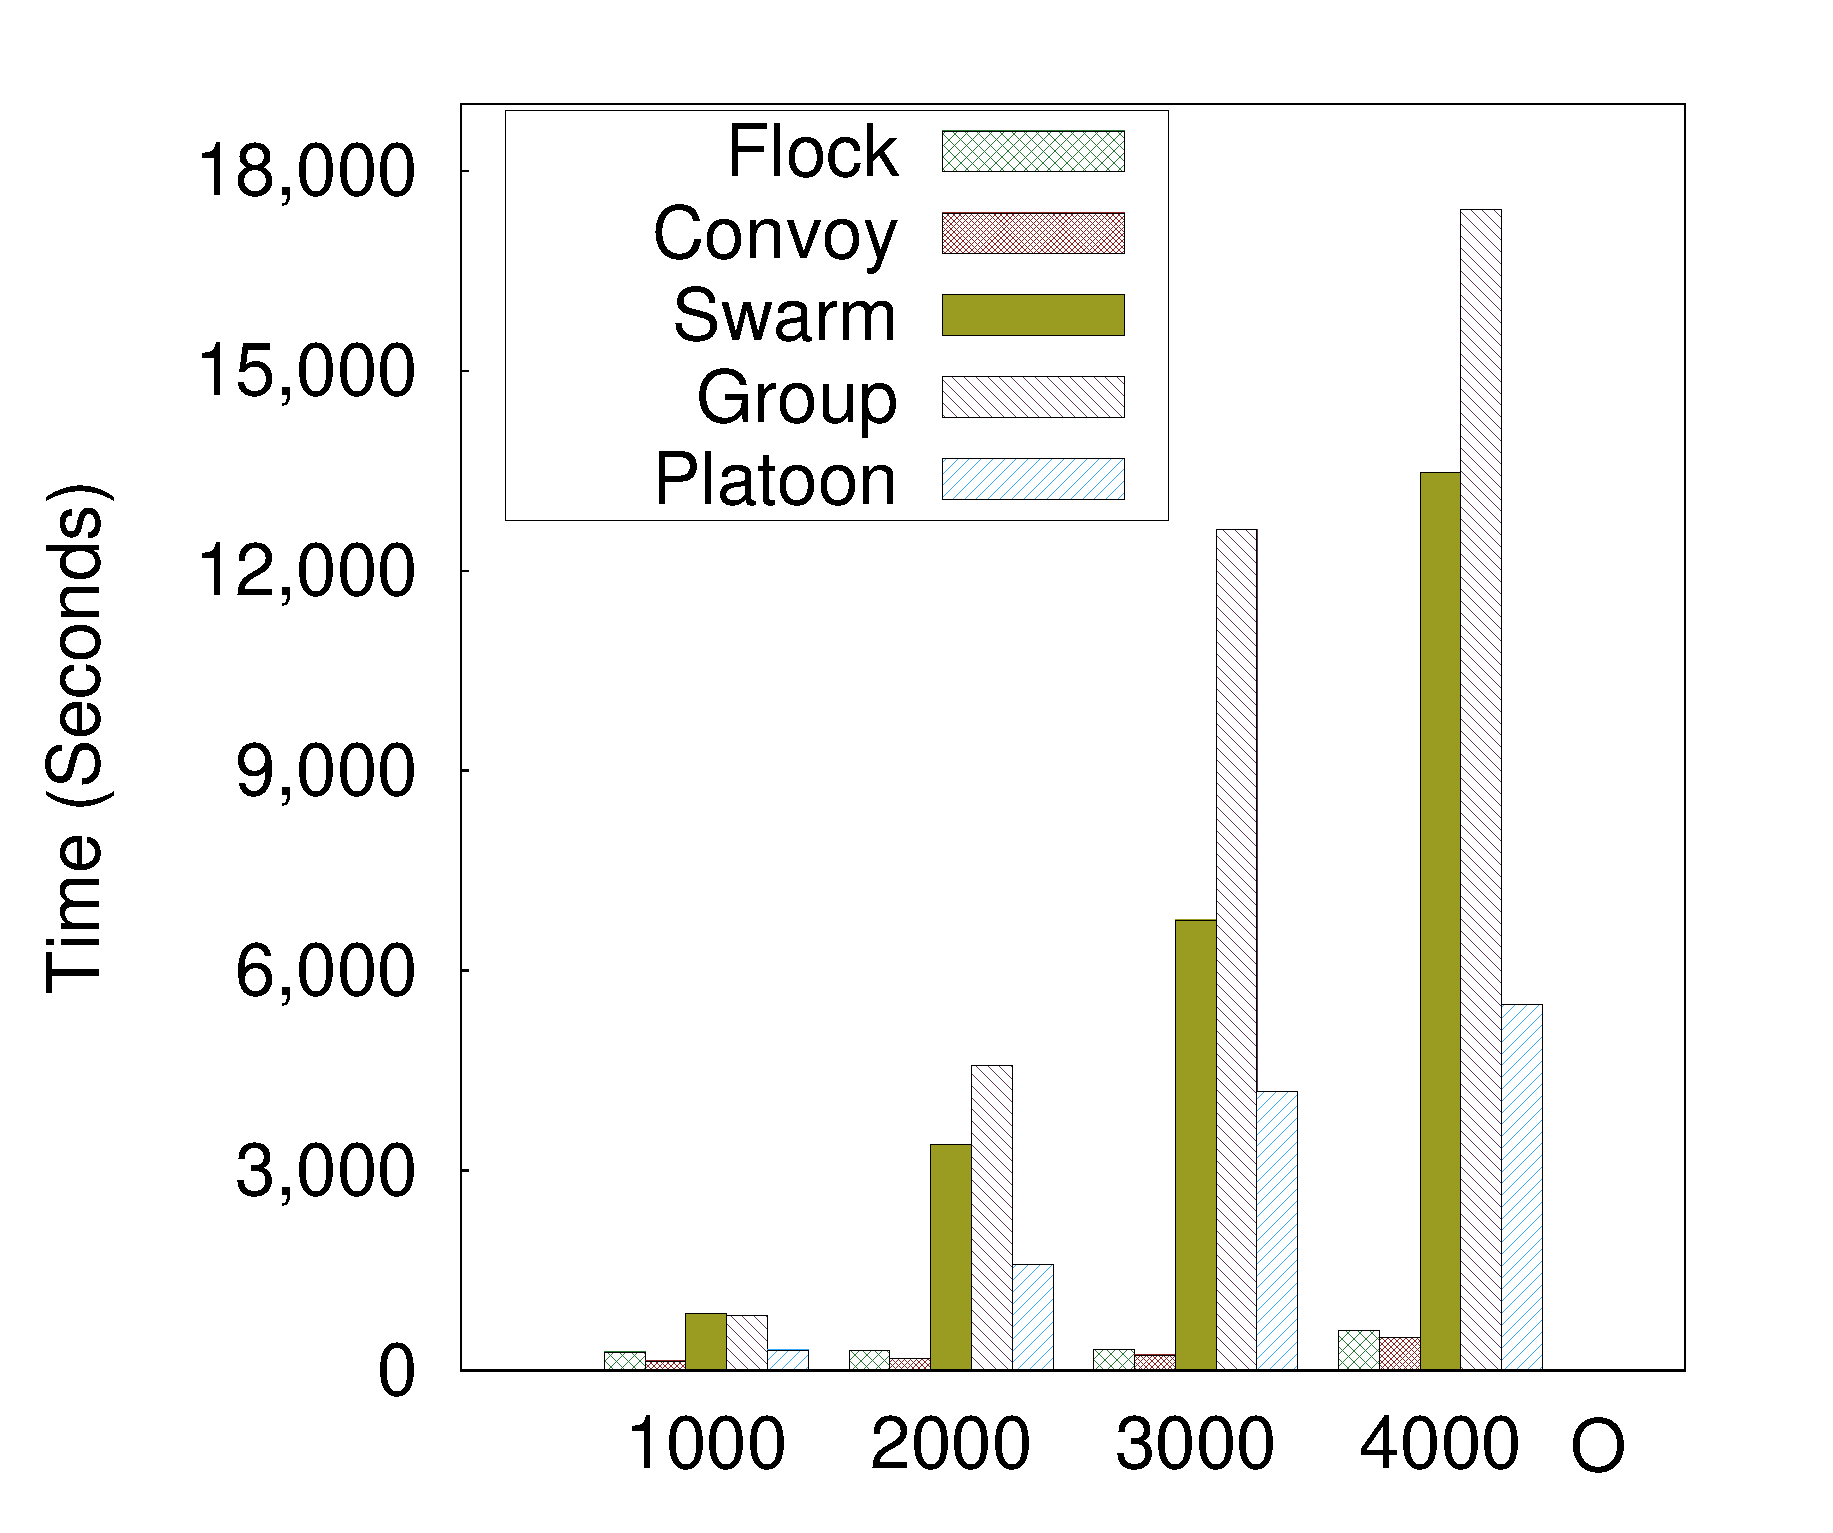
\includegraphics[width=0.35\textwidth]{rw_perf_O.eps}
%\caption{Two anomalies in existing patterns. (a) \emph{Missing-pattern} anomaly
%in \emph{flock} and \emph{convoy}. When $K=4$, none of the two patterns can be discovered. (b) \emph{Loose-connection} anomaly in \emph{platoon} and \emph{swarm}. The consecutive segment of $o_1$ and $o_2$ are 98 timestamps apart, however, the pattern $\{o_1, o_2: 1,2,3,102,103,104\}$ is included in platoon and swarm results.}
%\label{fig:platoon_weakpoint}
%\end{figure}


The other issue with existing methods is that they are built on top of centralized indexes which may not be scalable. Table~\ref{tbl:existing_co_patterns} shows their theoretical complexities in the worst cases and the largest real dataset ever evaluated in previous studies is up to million-scale points collected from hundreds of moving objects. In practice, the dataset is of much higher scale and the scalability of existing methods is left unknown. Thus, we conduct an experimental evaluation with $4000$ objects moving for $2500$ timestamps to examine the scalability. Results in Figure~\ref{fig:related_work_scalability} show that their performances degrade dramatically as the dataset scales up. For instance, the detection time of \emph{group} drops twenty times as the number of objects grows from \emph{1k} to \emph{4k}. Similarly,
the performance of \emph{swarm} drops over fifteen times as the number of snapshots grows from \emph{1k} to \emph{2.5k}.
These observations imply that existing methods are not scalable to support large-scale trajectory databases. 

%It is easy to spot that none of the existing solutions are scalable to handle large-scale trajectories which include near billions of data points.
%In fact, as shown in Table~, the mining of co-movement patterns require high complexity. For instance, the
%complexities of \emph{swarm} and \emph{platoon} are already exponential. 
%Therefore, none of them can handle millions of trajectories efficiently. 
%CAN YOU ANALYSE THEIR COMPLEXITY TO ADDRESS THE PROBLEM OF SCALABILITY.
\begin{figure}[h]
    \centering
    \begin{subfigure}[b]{0.23\textwidth}
            \centering
            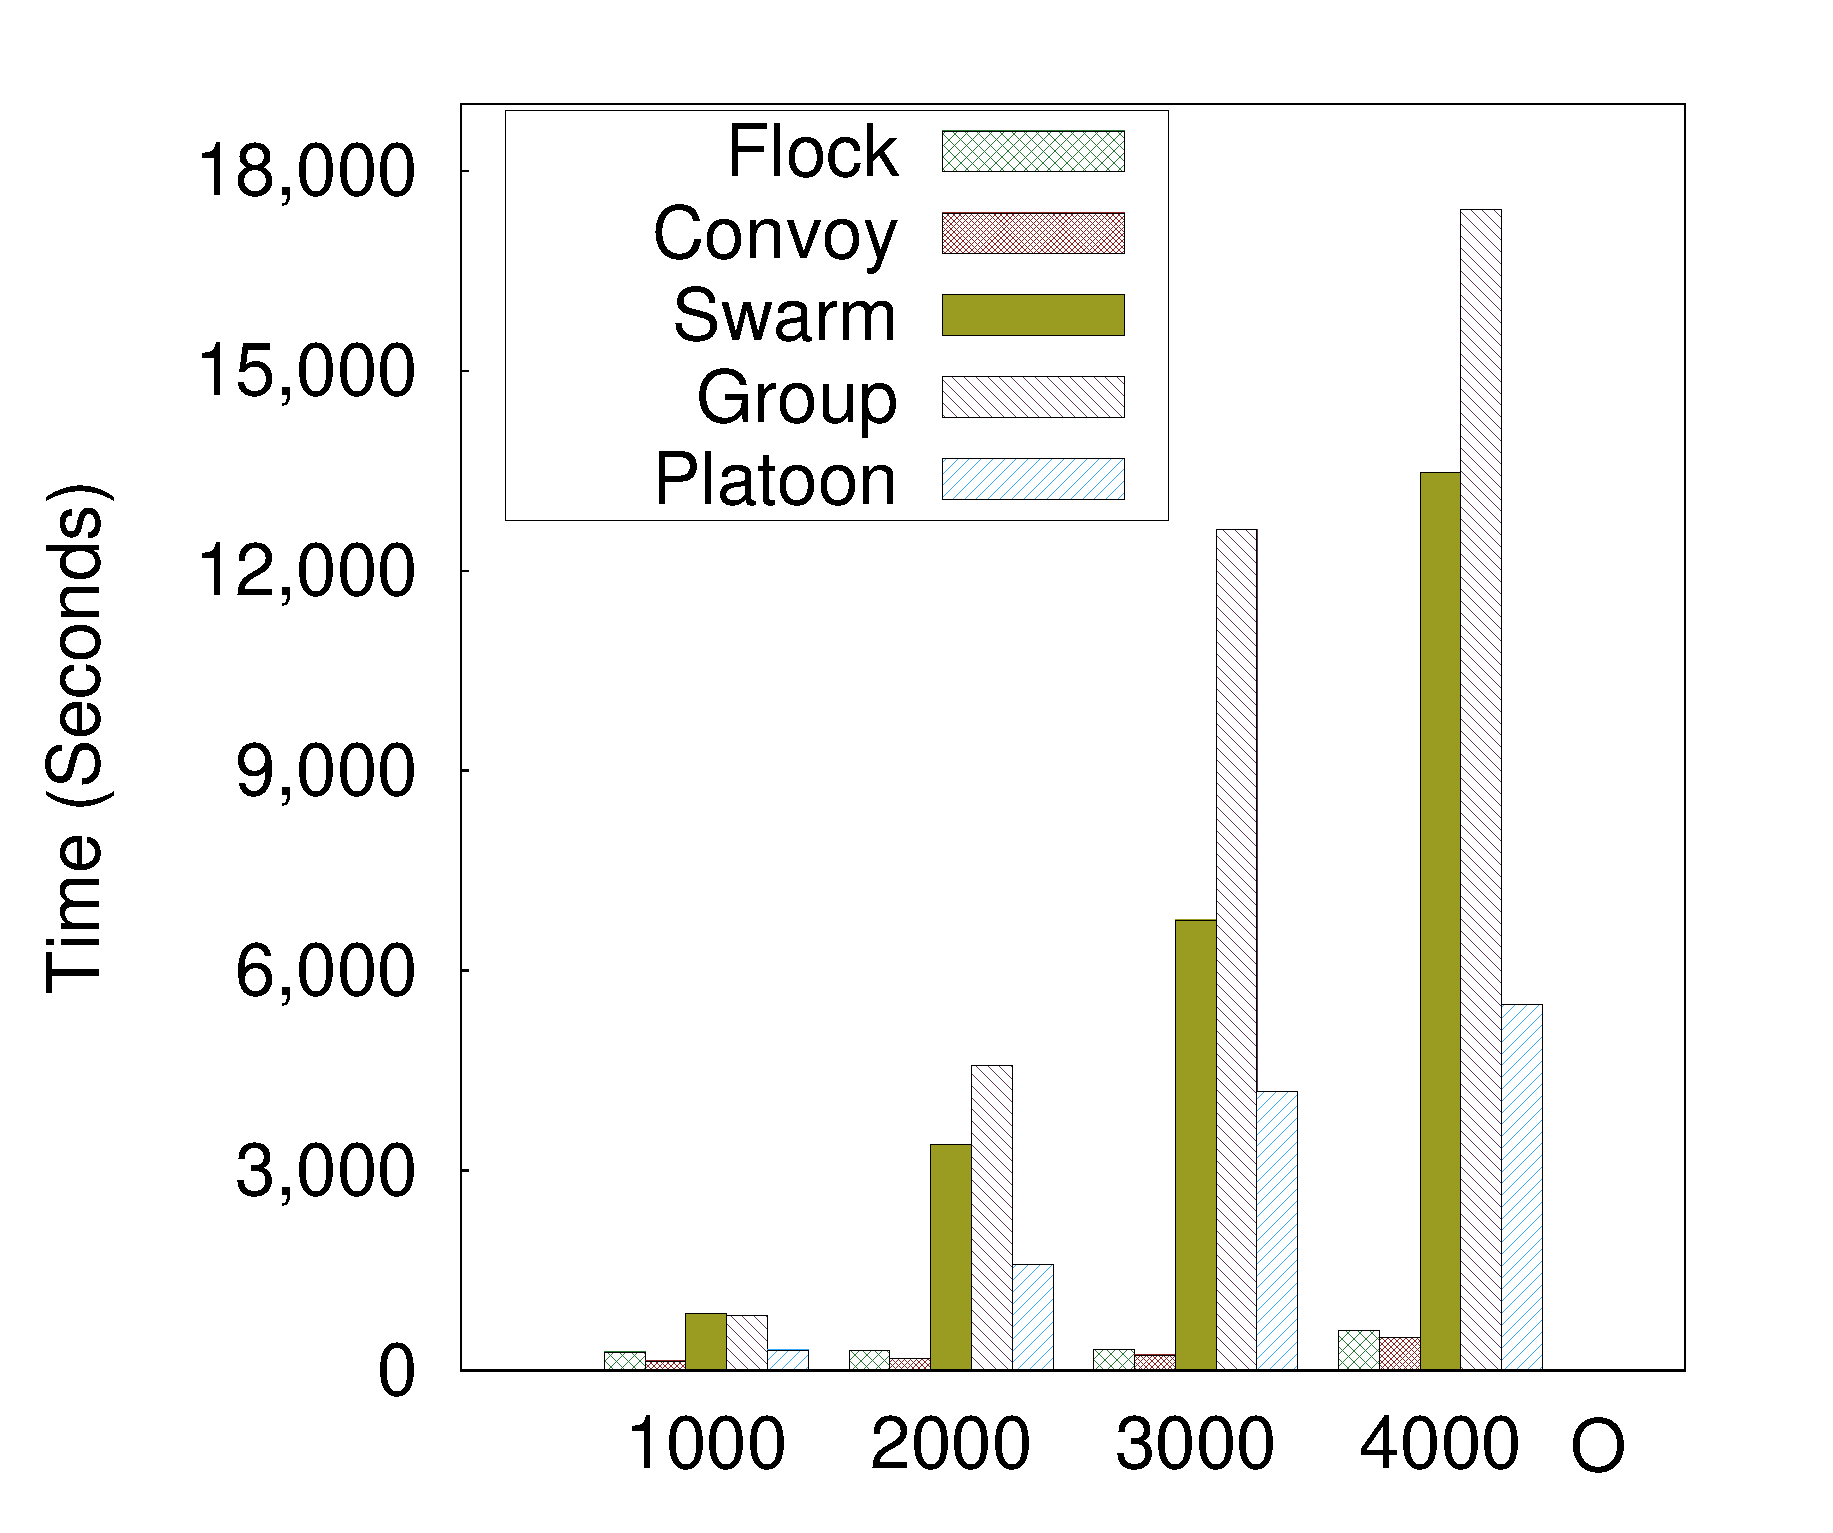
\includegraphics[width=\textwidth]{rw_perf_O.eps}
		\subcaption{$1k$ timestamps}
    \label{fig:fig1}
    \end{subfigure}
    \begin{subfigure}[b]{0.23\textwidth}
            \centering
            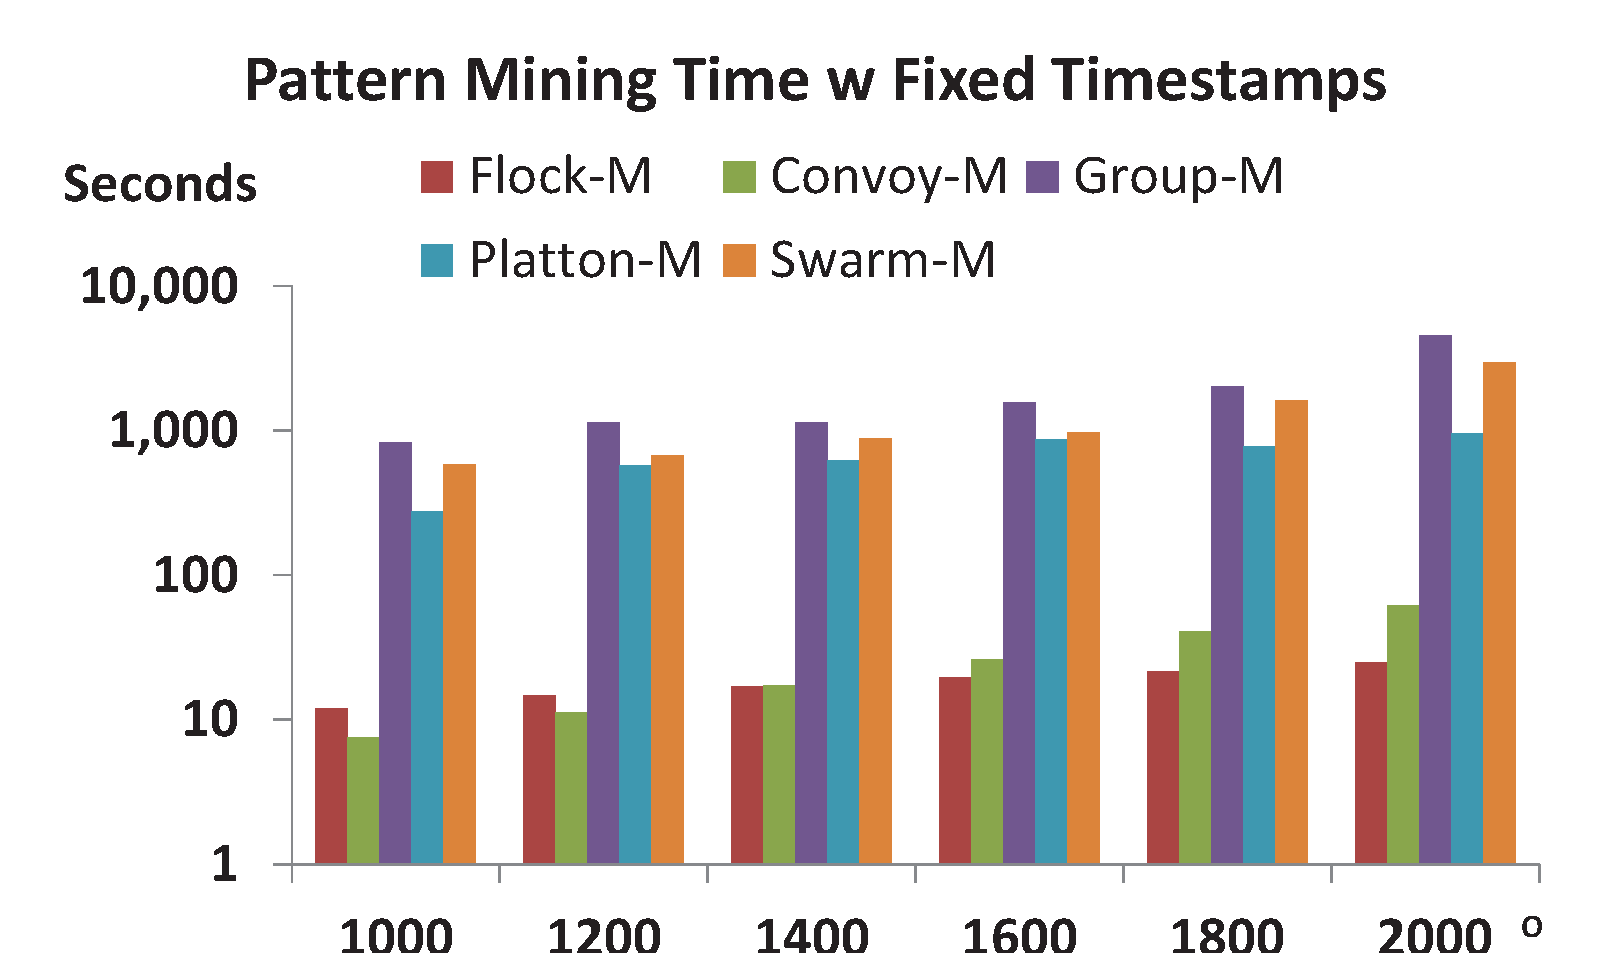
\includegraphics[width=\textwidth]{rw_perf_T.eps}
         \subcaption{$1k$ objects}
    \label{fig:fig2}
    \end{subfigure}
    \caption{Performance measures on existing co-movement patterns. A sampled Geolife data set
    is used with up two 2.4 million data points. Default parameters are $M=10$ $K=20$ $L=10$.}
    \label{fig:related_work_scalability}
\end{figure}




Therefore, our primary contributions in this paper are to close these two gaps. 
First, we propose the \emph{general co-movement pattern} (GCMP) which models
various co-moment patterns in a unified way and can avoid 
the \emph{loose-connection} anomaly. In GCMP, we introduce a new gap parameter $G$ to pose a constraint on the temporal gap between two consecutive segments. By setting a feasible $G$, the loose-connection anomaly can be avoided. In addition, our GCMP is both general and expressive. It can be reduced to any of the previous patterns by customizing the parameters.

%Therefore, users are 
%still able to exclude non-consecutive patterns 
%or include loosely-connected patterns when they feel necessary.


%We introduce the gap parameter $G$,
%When such loosely-connected patterns are unwanted, users currently are unable to directly control the outputs.
%To cope with both of the two anomalies, we propose 
%by introducing the gap parameter $G$, 

%By so doing, we gain a fine-grained control s, which As we show in later sections, the general co-movement pattern is able to express existing patterns by setting appropriate parameters. 
%IS IT POSSIBLE TO USE FIGURE 1 TO ADDRESS THE PROBLEM OF PLATOON, INSTEAD OF PROPOSING A NEW EXAMPLE SCENARIO?
%

Second, we investigate deploying our GCMP detector on MapReduce platforms (such as Hadoop and Spark) to tackle the scalability issue. Our technical contributions are three-fold. First, we replicate the snapshots in multiple data chunks to support efficient parallel processing. Second, we devise a novel \emph{Star Partition and Mining} (SPM) algorithm as a fine-granularity partitioning strategy to achieve workload balance. For each star, an Apriori method is adopted to mine the co-movement patterns. Third, we propose two types of optimization techniques to further improve the performance, including \emph{edge-simplification} to boost the shuffle process and \emph{temporal monotonicity pruning} and 
\emph{forward closure checking} to significantly reduce the number of enumerated candidates in the Aproiro algorithm.



%
%Second, we investigate on deploying our GCMP detector to facilitate scalable pattern mining.
%In order to support large real trajectories, to the best of our knowledge, we
%are the first to study GCMP mining in MapReduce (MR) systems. There are a
%few challengers associated with designing an efficient MR-based pattern 
%detection algorithms. 
%
%First, in order to support effective parallelism, we need
%to partition the trajectory database with almost equal sizes. Our initial attempts
%develops a temporal based partition approached named as 
%\emph{Temporal Replication and Mining} (TRM). In TRM, neighboring snapshots form
%a equal-sized partition such that co-movement patterns can be mined independently.
%However, such a scheme require $O(|\mathbb{T}|)$ replication of input, which is 
%inefficient for large-scale trajectories. To support efficient mining, 
%we design a novel \emph{Star Partition and Mining} (SPM) approach which utilize
%the potential co-movement relationship among objects.
%
%Our initial attempt develops a naive but effective 
%\emph{Temporal Replication and Mining} (TRM) approach 
%which requires to replicate entire data set $O(|\mathbb{T}|)$ times. Such a 
%large set of 

%There
%are a few challenges arises in designing the MR based pattern detection algorithm.
%First, we 

%The major challenge
%we face is to make proper data partitions such
%that each partition can be efficiently processed independently. Our initial attempt develops
%a naive but effective \emph{Temporal Replication and Mining} (TRM) approach which requires to replicate
%entire data set $O(|\mathbb{T}|)$ times. To improve the efficiency, we design a novel \emph{Star Partition and Mining} (SPM)
%algorithm. In SPM, potential co-moving objects are first grouped into partitions. Subsequently,
%an apriori based method is applied to discover the patterns from each partition.
%Despite the simpleness of the star partition, we theoretically prove its correctness
%and optimality. Using SPM as the foundation, we develop and integrate
%a series of optimization techniques including \emph{edge simplification}, \emph{candidate pruning}
%and \emph{forward closure checking} to further boost the
%performances.
%


%
%Second, we investigate how to deploy our GCMP detector  on Spark for scalable pattern mining.
%The major challenge in designing MapReduce-based algorithms is to make proper partitions of input data.
%In GCMP mining, we enforce both the \emph{soundness} and the \emph{completeness} 
%of the partitions. Such properties ensure that neither false-patterns 
%nor miss-patterns are possible in our solution. To meet such partition requirements
%as well as to keep the shuffle amount to a minimum, 
%we first design a naive \emph{Temporal Replication and Mining} (TRM)
%approach, which partitions trajectories into groups of consecutive snapshots. Then, we design a line-sweep
%method for mining GCMP from each partition. We prove that in TRM, the partition is complete and sound when a snapshot is replicated $O(|T|)$ times. 
%Then, we design a novel \emph{Star Partition and Mining} (SRM) approach which significantly reduces the data shuffled
%as compare to TRM. In SRM, we design a conceptual connection graph based on proximity among objects. We adapt
%a \emph{star partition} which cut the graph by replicating vertices. Afterwards, we design an Apriori-like method to mine
%GCMP in each partition. We prove the correctness of SPM and show that total data been replicated is $O(|\mathbb{O}|)$. 
%Despite the simpleness of star partition, we theoretically prove its optimality.
%Furthermore, we utilize \emph{temporal monotonicity} to further reduce the 
%shuffling and mining cost in SPM. 
%Lastly, we adapt various engineering level techniques to support efficiently deploying our algorithms in 
%Apache Spark which is one of the most popular MapReduce platforms.

%we design a novel star-based partition scheme to efficiently partition objects based on their
%belonging clusters. Based on the star partition, we then propose a series of optimization techniques which
%largely improve the system performance. NEED TO EMPHASIZE YOUR TECHNICAL CONTRIBUTION!

We conduct a set of extensive experiments on XXX datasets with billion-scale trajectory points. The results show that XXX.

The rest of our paper is organized as follows: Section~\ref{sec:related_works} summarizes the relevant literature on 
trajectory pattern mining. Section~\ref{sec:definition} states the problem definition of our general co-movement pattern mining. Section~\ref{sec:trm} provides a naive \emph{temporal replication and mining} solution. An advanced solution named
\emph{star partition and mining} is presented in Section~\ref{sec:spm}. Section~\ref{sec:opt} discusses various optimization techniques. Section~\ref{sec:exp} conducts extensive experiments to verify the usefulness and efficiency of our system. Finally Section~\ref{sec:concl} concludes the paper.
